% Dmitry Mikushin, Applied Parallel Computing LLC, dmitry@kernelgen.org

\documentclass[aspectratio=169,twoside]{beamer}

\usetheme{unil}
\usepackage{comment}
\usepackage{enumerate}
\usepackage{xcolor}
\usepackage{setspace}
\usepackage{mathrsfs}
\usepackage{multibbl}
\usepackage{relsize}
\usetikzlibrary{calc,shapes.callouts,shapes.arrows}

\makeatletter
\newcommand{\changeoperator}[1]{%
  \csletcs{#1@saved}{#1@}%
  \csdef{#1@}{\changed@operator{#1}}%
}
\newcommand{\changed@operator}[1]{%
  \mathop{%
    \mathchoice{\textstyle\csuse{#1@saved}}
               {\csuse{#1@saved}}
               {\csuse{#1@saved}}
               {\csuse{#1@saved}}%
  }%
}
\makeatother

\newcommand{\tsubame}[1]{
\tikz[remember picture,baseline]{
\node[xshift=1.7cm,yshift=-1cm,overlay,rectangle callout,callout relative pointer={(-0.3cm,0.7cm)},fill=white,draw=unil@blue,inner sep=4pt,outer sep=0, align=center, execute at begin node=\setlength{\baselineskip}{0.7em}] at (current page.center)
{#1};
}}%

\newcommand{\pizdaint}[1]{
\tikz[remember picture,baseline]{
\node[xshift=5.1cm,yshift=-0.05cm,overlay,rectangle callout,callout relative pointer={(-0.3cm,0.7cm)},fill=white,draw=unil@blue,inner sep=4pt,outer sep=0, align=center, execute at begin node=\setlength{\baselineskip}{0.7em}] at (current page.center)
{#1};
}}%

\title[Multi-iterator Engine]{Multi-iterator Engine}
\author[Dmitry Mikushin et al.]{Dmitry Mikushin\quad Simon Scheidegger\quad Philipp Eisenhauer\quad Moritz}
\institute[UNIL]{}
\date{May 4, 2021}



\begin{document}



{
\setbeamertemplate{footline}{} 
\begin{frame}
  \titlepage
\end{frame}
}
\addtocounter{framenumber}{-1}



\setbeamercovered{transparent=5}



\begin{frame}[fragile]{Multi-Iterator: the purpose}

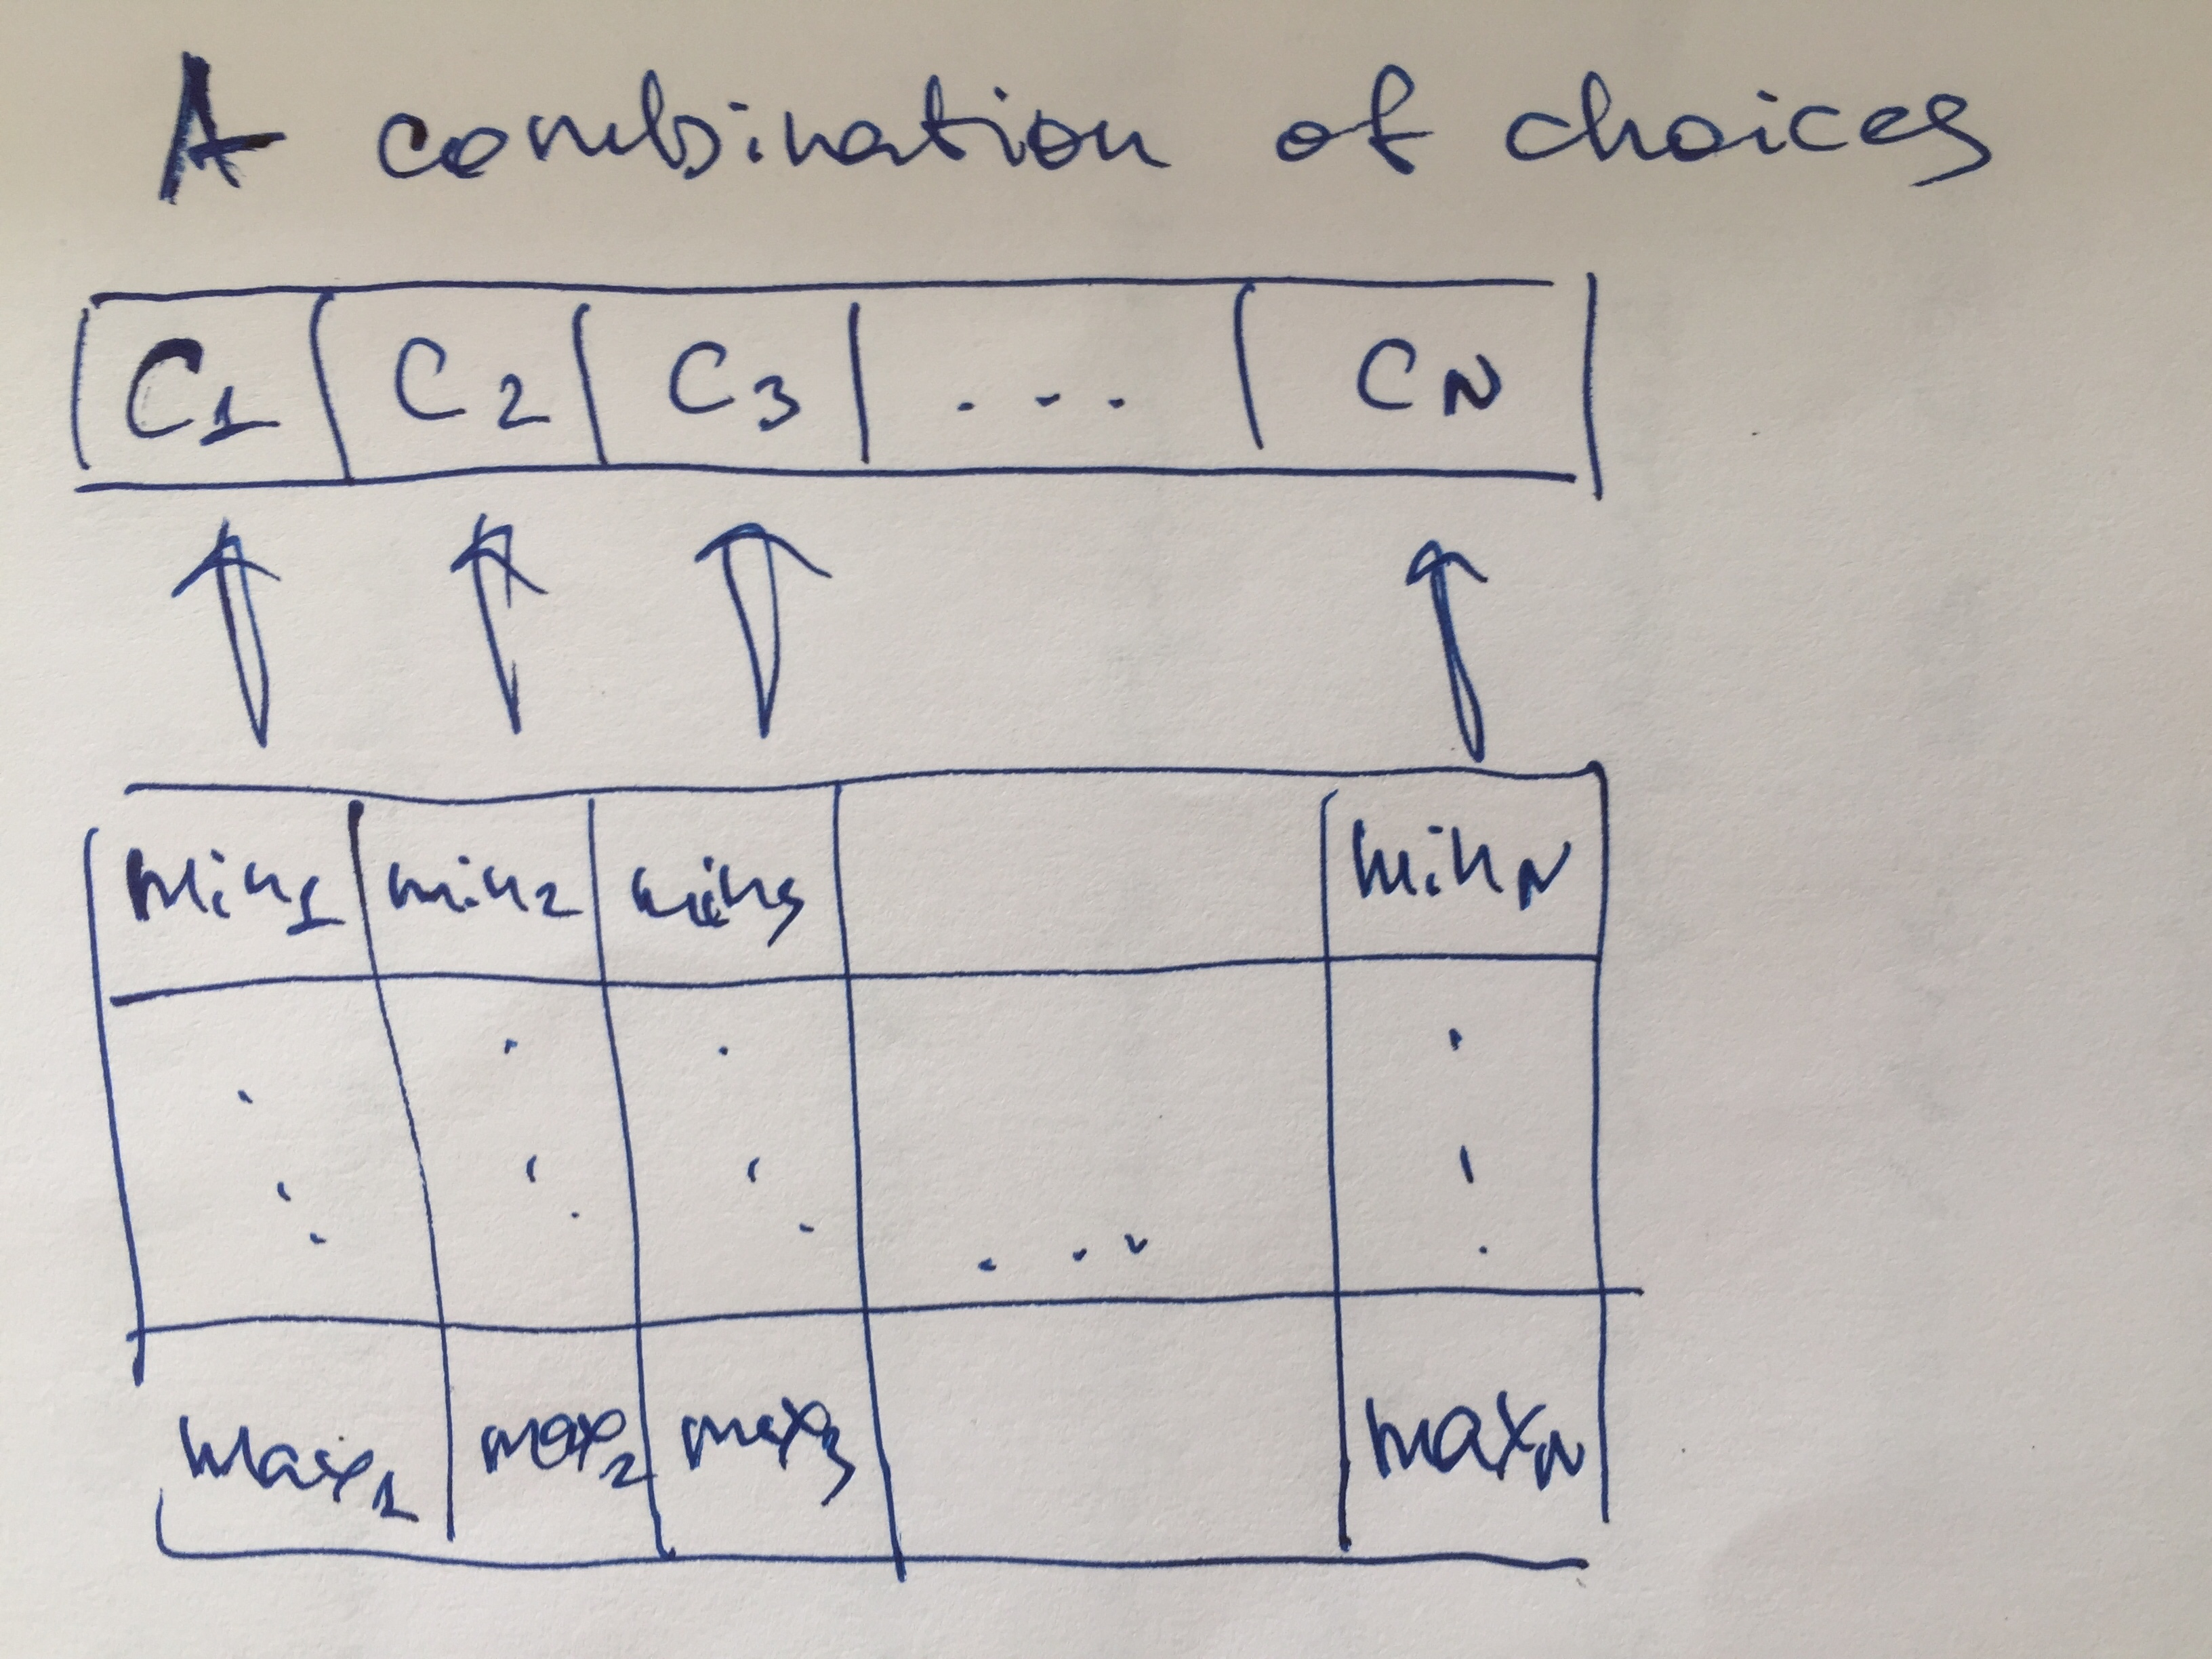
\includegraphics[width=7cm]{figures/IMG_0509}

\end{frame}



\begin{frame}[fragile]{Simple example}

\begin{lstlisting}[basicstyle=\tiny\ttfamily, language=c++]
#include <multiit/multiit.h>

multiit::runtime::MultiIterator mi({ 2, 3, 4 });
// OR: multiit::compiletime::MultiIterator<2, 3, 4> mi;

int niters = 0; 
while (1)       
{               
    niters++;           
                        
    bool next = mi.next();
    if (!next) break;   
                        
    const auto& current = mi.getCurrent();
                        
    // TODO Use the current combination of choices in a target app.
}               

printf("%d iterations visited\n", niters);
\end{lstlisting}

\end{frame}



\begin{frame}[fragile]{Supported types of multi-iterators}

\begin{itemize}
\item \texttt{MultiIterator}: A group of indexes that iterate from 0 to the given upper value
\item \texttt{LimitedMultiIterator}: A group of indexes that iterates only through indexes with total sum no greater than limit
\item \texttt{GenericMultiIterator}: A group of indexes, whose indexes are themselves groups of indexes
\end{itemize}

\end{frame}



\end{document}

